\documentclass[../main.tex]{subfiles}

\begin{document}

\justifying

\section{Ver que onda el potencial de tres cuerpos.}

\paragraph{Obejtivo:} Comprobar que la tabulación del potencial de 3 cuerpos es correcto.

\subsection{Descripción de la simulación}

\begin{marginfigure}
    \caption{\(t=0\)}
    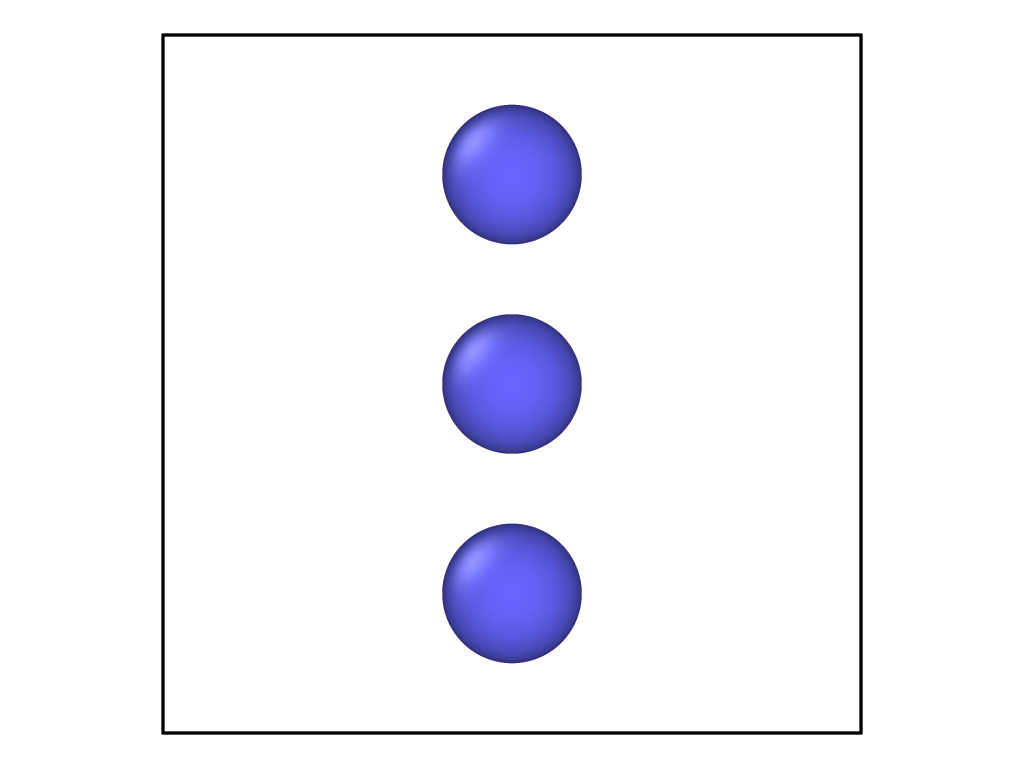
\includegraphics{../Figures/tests2/t_0.png}
\end{marginfigure}
\begin{marginfigure}
    \caption{\(t=4.5\)}
    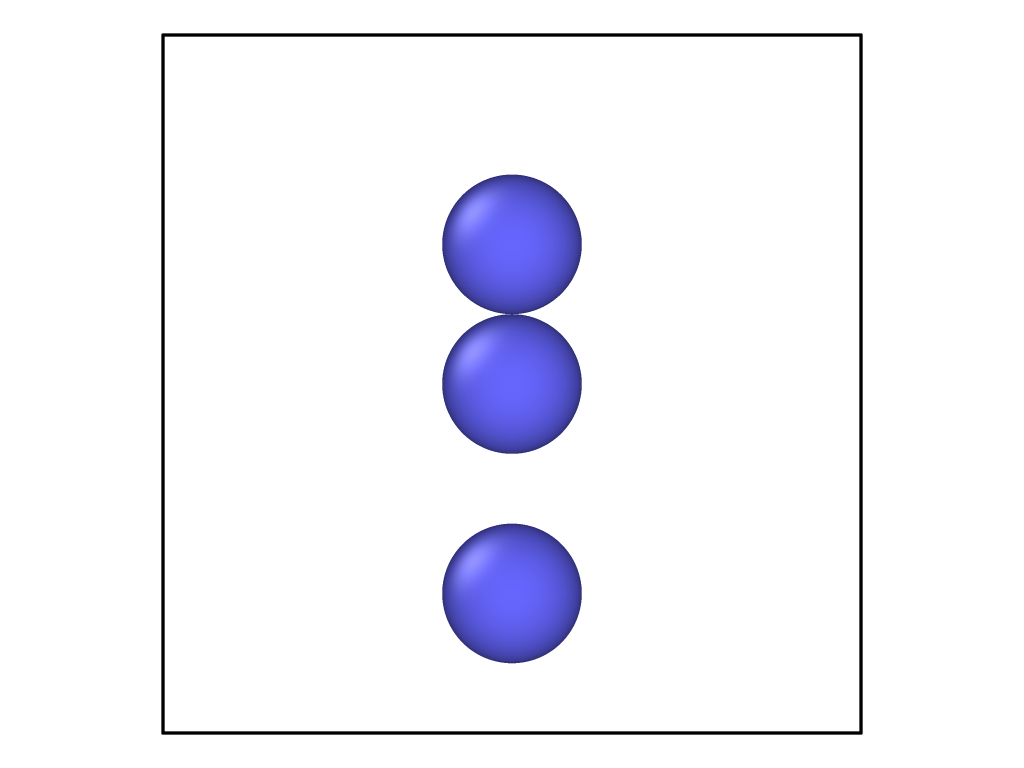
\includegraphics{../Figures/tests2/t_2.png}
\end{marginfigure}
\begin{marginfigure}
    \caption{\(t=9\)}
    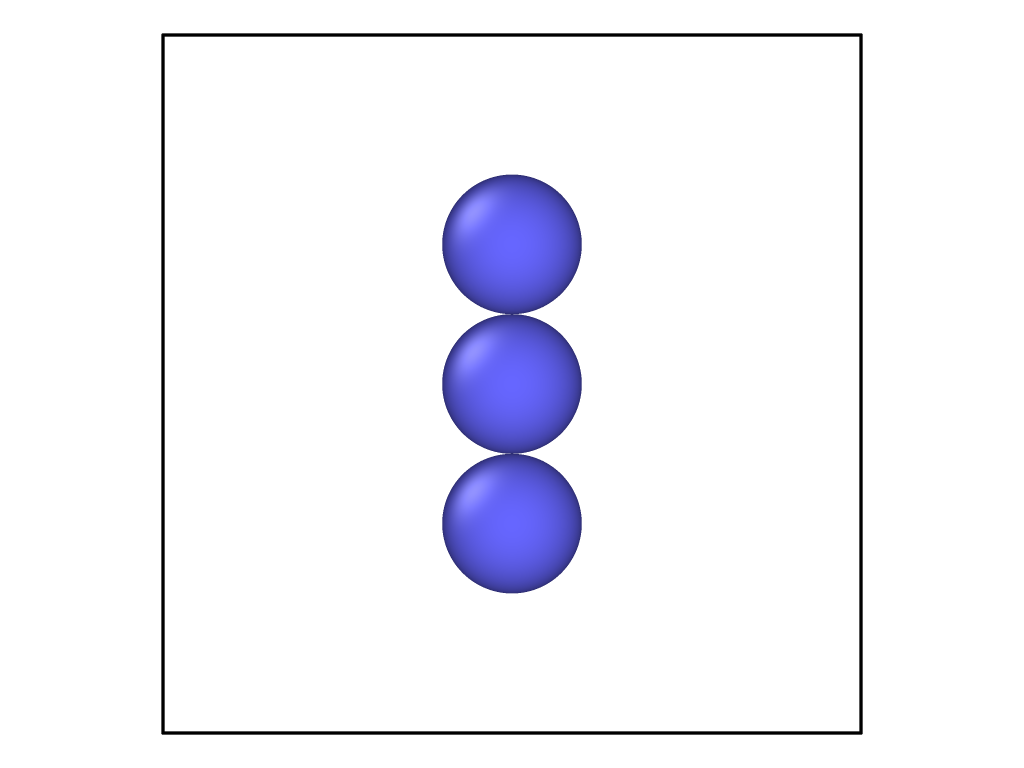
\includegraphics{../Figures/tests2/t_4.png}
\end{marginfigure}

Se colocan 3 partículas.
Una partícula en el centro \(\vec{r}_1 = (0,0,0)\).
Una segunda partícula en \(\vec{r}_2 = (0,0.6,0)\).
Una tercera partícula en \(\vec{r}_3 = (0,-0.6,0)\).
Primero se mueve la partícula 2 hacia la partícula central con velocidad \(\vec{v}_2=(0,-0.1,0)\).
Cuando la segunda partícula llegué a \(0,0.4,0.0\) se detiene el movimiento (\num{2000} pasos).
Posteriormente se mueve la tercera partícula con velocidad \(\vec{v}_3=(0,0.1,0)\) hasta qu llegué a la posición \(0,-0.4,0\) (\num{2000} pasos).

\newpage

\section{Directory: 2026-02-23-111821}

\begin{figure}[!ht]
    \centering
    
\includegraphics[width=0.8\textwidth]{../Figures/2026-02-23-111821/fig_FComp.png}
    \caption{Fuerza en cada partícula.
        Línea azul: particula central.
        Línea naranja: partícula superior.
        Línea verda: partícula verde.
    }\label{fig:ForceSwapComponentsNew}
\end{figure}

\begin{figure}[!ht]
    \centering
    
\includegraphics[width=0.8\textwidth]{../Figures/2026-02-23-111821/fig_ForceSwapcomp.png}
    \caption{Fuerza en cada partícula.
        Línea azul: particula central.
        Línea naranja: partícula superior.
        Línea verda: partícula verde.
    }\label{fig:ForceSwapComponentsNew}
\end{figure}




\newpage

\section{Ver que onda el potencial de tres cuerpos.}

\paragraph{Objetivo:}  Ver las configuraciones en las que el pontencial de 3 cuerpos funciona.

\subsection{Descripción de la simulación}

\begin{marginfigure}
    \caption{\(t=0\)}
    
\includegraphics{../Figures/test3/triangle-1.png}
\end{marginfigure}
\begin{marginfigure}
    \caption{\(t=2\)}
    
\includegraphics{../Figures/test3/triangle-2.png}
\end{marginfigure}
\begin{marginfigure}
    \caption{\(t=4\)}
    
\includegraphics{../Figures/test3/triangle-3.png}
\end{marginfigure}

Se colocan 3 partículas.
Una partícula en el centro \(\vec{r}_1 = (0,0,0)\).
Una segunda partícula en \(\vec{r}_2 = (0,0.6,0)\).
Una tercera partícula en \(\vec{r}_3 = (0.6,0,0)\).
Primero se mueve la partícula 2 hacia la partícula central con velocidad \(\vec{v}_2=(0,-0.1,0)\).
Cuando la segunda partícula llegué a \(0,0.4,0.0\) se detiene el movimiento (\num{2000} pasos).
Posteriormente se mueve la tercera partícula con velocidad \(\vec{v}_3=(-0.1,0,0)\) hasta qu llegué a la posición \(0.4,0,0\) (\num{2000} pasos).

\newpage

\section{Directory: 2026-02-23-112958}


\begin{figure}[!ht]
    \centering
    
\includegraphics[width=0.8\textwidth]{../Figures/2026-02-23-112958/fig_FComp.png}
    \caption{Fuerza en cada partícula.
        Línea azul: particula central.
        Línea naranja: partícula superior.
        Línea verda: partícula verde.
    }\label{fig:ForceSwapComponentsNew}
\end{figure}

\begin{figure}[!ht]
    \centering
    
\includegraphics[width=0.8\textwidth]{../Figures/2026-02-23-112958/fig_ForceSwapcomp.png}
    \caption{Fuerza en cada partícula.
        Línea azul: particula central.
        Línea naranja: partícula superior.
        Línea verda: partícula verde.
    }\label{fig:ForceSwapComponentsNew}
\end{figure}



%Cómo podemos observar, esta configuración no es válida para el potencial de 3 cuerpos, porqué el ángulo formado entre las partículas $i-j$, $i-k$ es mayor que \(\acos(\dfrac{1}{3})\)

%Se cambiará la configuración del experimento.

\newpage

\section{Ver que onda el potencial de tres cuerpos.}

\paragraph{Objetivo:}  Ver las configuraciones en las que el pontencial de 3 cuerpos funciona.

\subsection{Descripción de la simulación}

\begin{marginfigure}
    \caption{\(t=0\)}
    
\includegraphics{../Figures/test3_a/triangle-1.png}
\end{marginfigure}
\begin{marginfigure}
    \caption{\(t=2\)}
    
\includegraphics{../Figures/test3_a/triangle-2.png}
\end{marginfigure}
\begin{marginfigure}
    \caption{\(t=5\)}
    
\includegraphics{../Figures/test3_a/triangle-3.png}
\end{marginfigure}

Se colocan 3 partículas.
Una partícula en el centro \(\vec{r}_1 = (-0.2,0,0)\).
Una segunda partícula en \(\vec{r}_2 = (0.4,0,0)\).
Una tercera partícula en \(\vec{r}_3 = (0.0,0.646410,0)\).
Primero se mueve la partícula 2 hacia la partícula central con velocidad \(\vec{v}_2=(-0.1,0,0)\).
Cuando la segunda partícula llegué a \(0.2,0,0.0\) se detiene el movimiento (\num{2000} pasos).
Posteriormente se mueve la tercera partícula con velocidad \(\vec{v}_3=(0,-0.1,0)\) hasta que llegué a la posición \(0,0.346410,0\) (\num{3000} pasos).

\newpage

\section{Directory: 2026-02-23-120646}

\begin{figure}[!ht]
    \centering
    
\includegraphics[width=0.8\textwidth]{../Figures/2026-02-23-120646/fig_FComp.png}
    \caption{Fuerza en cada partícula.
        Línea azul: particula central.
        Línea naranja: partícula superior.
        Línea verda: partícula verde.
        Línea sólid: $x$,
        Línea punteada: $y$.
    }\label{fig:ForceSwapComponentsNew}
\end{figure}


\begin{figure}[!ht]
    \centering
    
\includegraphics[width=0.8\textwidth]{../Figures/2026-02-23-120646/fig_ForceSwapcomp.png}
    \caption{Fuerza en cada partícula.
        Línea azul: particula central.
        Línea naranja: partícula superior.
        Línea verda: partícula verde.
        Línea sólid: $x$,
        Línea punteada: $y$.
    }\label{fig:ForceSwapComponentsNew}
\end{figure}

\newpage

Estos experimentos indican que las fuerzas en el sistema obtenidas analíticamente y por LAMMPS son conscistentes.
Por otro lado, podemos observar, analisando la descripción analítica, que las dos primeras configuraciones no siguen la tercera ley de Newton.
Por otro lado, LAMMPS realiza los ajustes adecuados para que la tercera ley de newton se cumpla en cada partícula para todas las configuraciones.




\end{document}
